\section{Robot kinematic}

The robot kinematic is based on the motion model. 
\begin{definition}[\textit{Wheeled mobile robots}]
    A robot capable of locomotion on a surface solely through the actuation of wheel assemblies mounted on the robot and in contact with the surface. 
    A wheel assembly is a device which provides or allows motion between its mount and surface on which it is intended to have a single point of rolling contact.
\end{definition}

Various kinematic configurations are feasible:
\begin{itemize}
    \item \textit{Differential drive} (two wheels): basic design, prone to disturbances from uneven terrain, and lacks lateral translation capability.
    \item \textit{Tracks}: ideal for outdoor surfaces, movement precision compromised, especially during rotations, intricate structure and behavior, and lateral translation not achievable.
    \item \textit{Omnidirectional} (synchro drive): utilizes all three degrees of freedom, sophisticated design and functionality, and intricate structural composition.
\end{itemize}
\begin{figure}[H]
    \centering
    \begin{subfigure}{0.49\textwidth}
        \centering
        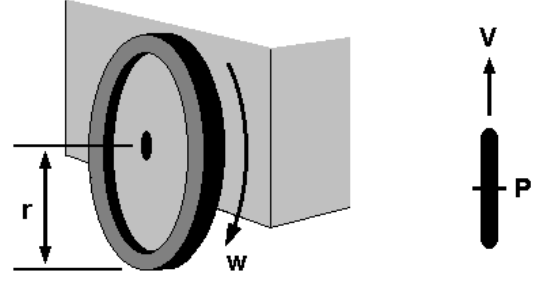
\includegraphics[width=0.5\linewidth]{images/fixed.png} 
        \caption{Fixed}
    \end{subfigure}
    \begin{subfigure}{0.49\textwidth}
        \centering
        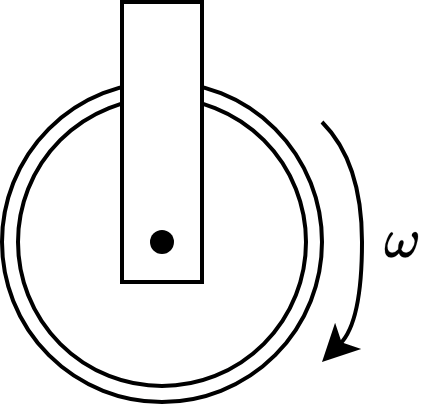
\includegraphics[width=0.5\linewidth]{images/oc.png}
        \caption{Orientable centered}
    \end{subfigure}
    \begin{subfigure}{0.49\textwidth}
        \centering
        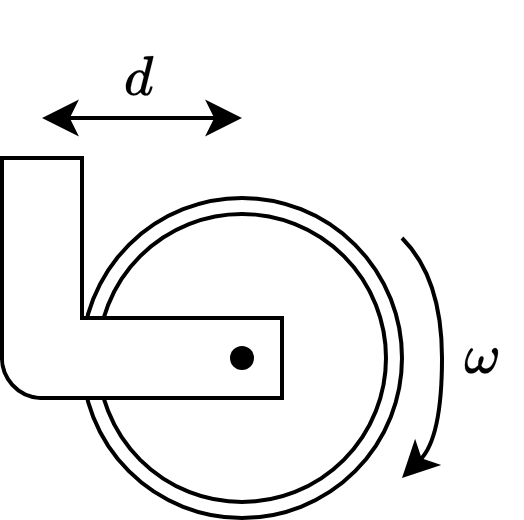
\includegraphics[width=0.5\linewidth]{images/co.png} 
        \caption{Caster omnidirectional}
    \end{subfigure}
    \begin{subfigure}{0.49\textwidth}
        \centering
        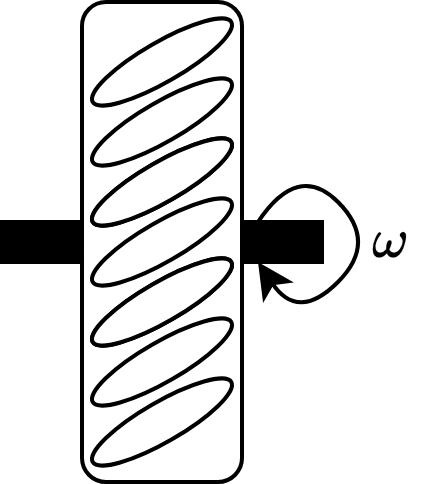
\includegraphics[width=0.5\linewidth]{images/sm.png}
        \caption{Swedish or meccanum}
    \end{subfigure}
    \caption{Wheel classification}
\end{figure}

\begin{definition}[\textit{Locomotion}]
    Locomotion involves initiating movement in an autonomous robot:
\end{definition}
Motion is achieved by applying forces to the vehicle.
\begin{definition}[\textit{Dynamics}]
    Dynamics encompasses the analysis of motion through the modeling of forces, as well as the associated energies and velocities involved in these movements.
\end{definition} 
\begin{definition}[\textit{Kinematics}]
    Kinematics is the examination of motion devoid of considerations regarding influencing forces. 
\end{definition}
It focuses on the geometric relationships dictating the system's behavior and the correlation between control parameters and the system's behavior in state space.

\begin{definition}[\textit{Direct kinematics}]
    Direct kinematics involves determining the pose $(x, y, \theta)$ that a robot achieves given specific control parameters and a time of movement $t$.
\end{definition}
\begin{definition}[\textit{Inverse  kinematics}]
    Inverse kinematics pertains to finding the control parameters necessary to reach a specified final pose $(x, y, \theta)$ within a given time $t$.
\end{definition}
\begin{figure}[H]
    \centering
    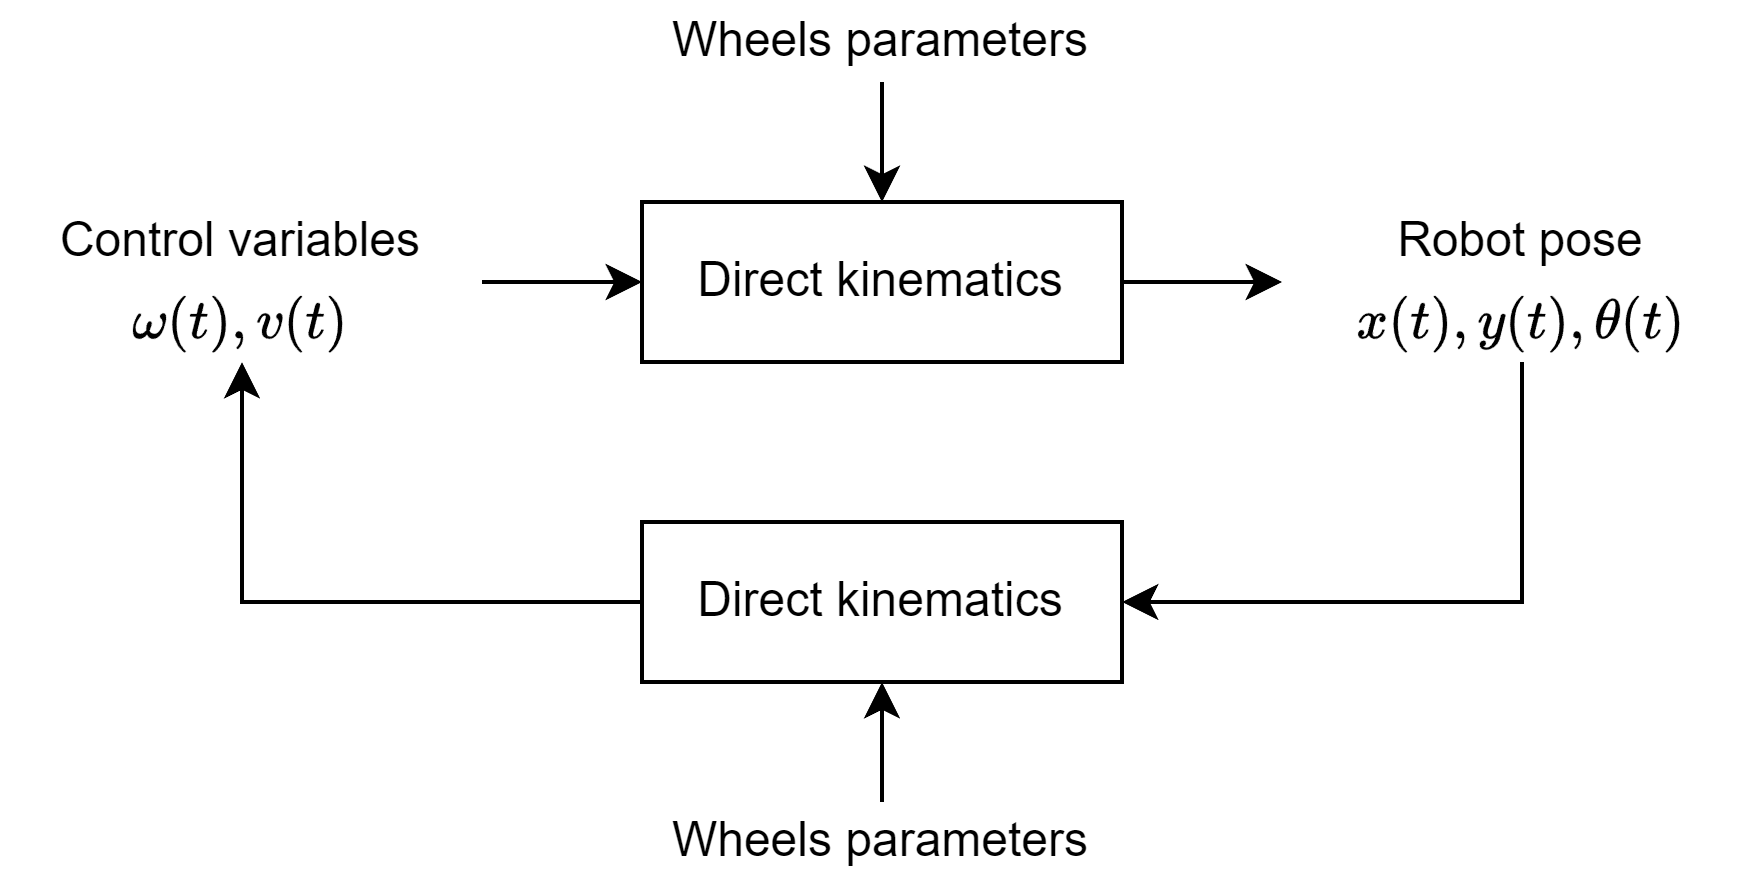
\includegraphics[width=0.75\linewidth]{images/kin.png} 
    \caption{Direct and inverse kinematics}
\end{figure}